\chapter{Erdös-Rényi model}
\label{cha: Erdös-Rényi model}
The Erdös-Rényi model is used to generate random graphs. It is a model that allows for the generation of graphs with a small diameter. This is a property that is also found in real networks. Contrary to real networks or the other models discussed in the lectures, it does not posses the property of high clustering nor it is scale-free. To plot the average shortest-path as a function of the network size the two variables for the Erdös-Rényi model G(n,p) have to be chosen accordingly. The graph from the task sheet uses zero to one million nodes and an unknown \textit{p} value. To calculate a suitable \textit{p} value that allows for a connected graph we use the following formulas from \cite{Erdos1984OnTE}.
\begin{itemize}
    \item If $ \,p < \frac{(1-\epsilon) \, ln \, n}{n} \,$ then a graph in G(n,p) will almost surely contain isolated vertices, and thus be disconnected.
    \item If $ \,p > \frac{(1-\epsilon) \, ln \, n}{n} \,$ then a graph in G(n,p) will almost surely be connected.
\end{itemize}
Because of insufficient hardware we had to reduce the maximum number of nodes \textit{n} that are considered to one hundred thousand instead of one million. Furthermore in the case that the graph is not fully connected we consider only the largest fully connected sub-graph. The graph from the task can not be recreated with a constant \textit{p} value for all values of \textit{n}. For example using a \textit{p} value of 0.1 for all values of \textit{n} results in the graph that can be seen in \ref{fig:ER Model with p = 0.1}.
We believe that using a rather large \textit{p} value of 0.1 leads to the creation of large central components in the graph once the \textit{n} value is adequately large. These central components lead to small shortest paths on average.
Therefore the value of \textit{p} has to be chosen in accordance of the value of \textit{n} to recreate the graph from the assignment. We have used the p value of $\,2\,ln(n)/n\,$, this is also recommended by the relevant literature to this topic. The resulting graph can be seen in \ref{fig:ER Model with dynamic P}. This graph shows that the average shortest path increases sharply with with the amount of nodes before reaching an stable value.
\begin{figure}
    \centering
    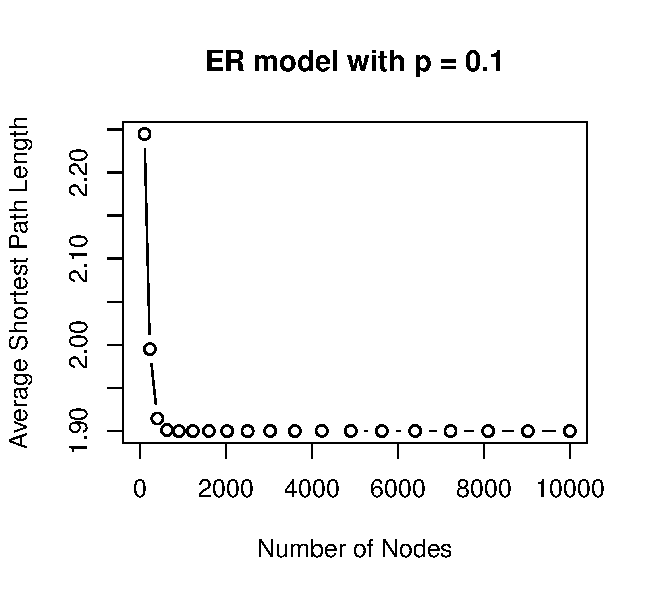
\includegraphics[width=0.66\textwidth]{figures/ER model with p = 0.1.pdf}
    \caption{ER model with a static \textit{p} of 0.1 and a maximal \textit{n} of 10000}
    \label{fig:ER Model with p = 0.1}
\end{figure}
\begin{figure}
    \centering
    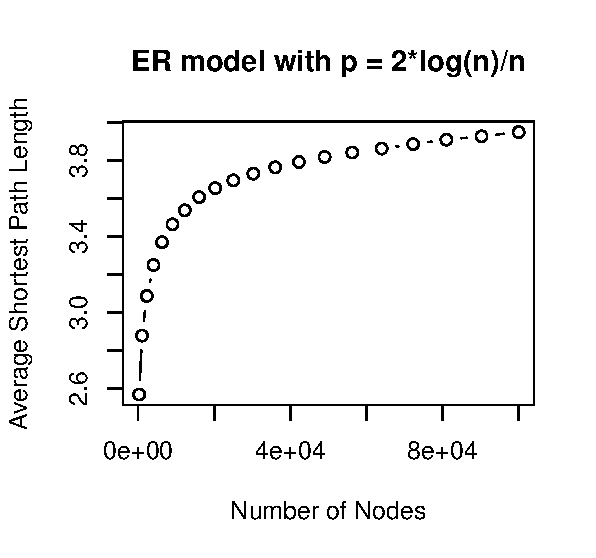
\includegraphics[width=0.66\textwidth]{figures/ermodelp2lognn100000.pdf}
    \caption{ER model with a dynamic \textit{p} of $\,2\,ln(n)/n\,$ and a maximal \textit{n} of 100000}
    \label{fig:ER Model with dynamic P}
\end{figure}